\documentclass[border=3pt]{standalone}
\usepackage{amsmath}
\usepackage{tikz}
\usetikzlibrary{arrows.meta,positioning,fit,backgrounds,calc}
\begin{document}
    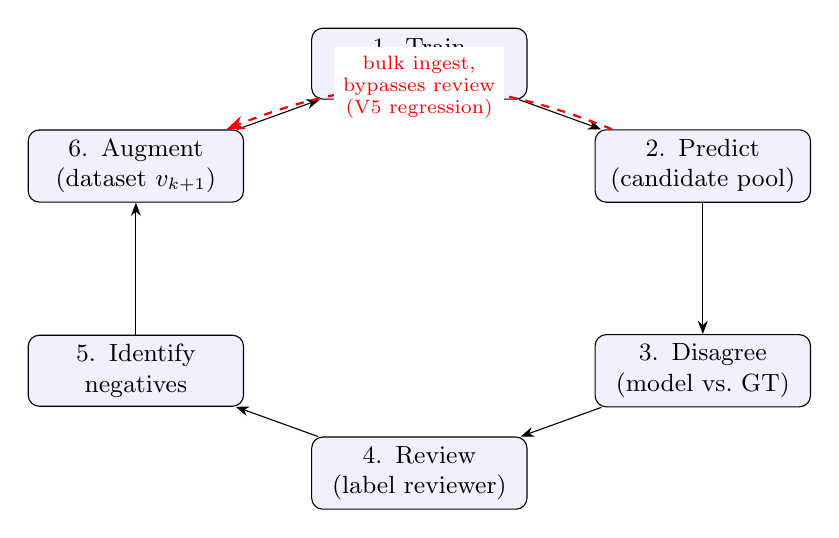
\begin{tikzpicture}[>=Stealth, font=\small,
      n/.style={draw, rounded corners, align=center, minimum height=9mm, text width=25mm, fill=blue!6}]
      \node[n] (train) at (0,2.6)    {1. Train\\model $v_k$};
      \node[n] (pred)  at (3.6,1.3)  {2. Predict\\(candidate pool)};
      \node[n] (dis)   at (3.6,-1.3) {3. Disagree\\(model vs.\ GT)};
      \node[n] (rev)   at (0,-2.6)   {4. Review\\(label reviewer)};
      \node[n] (neg)   at (-3.6,-1.3){5. Identify\\negatives};
      \node[n] (aug)   at (-3.6,1.3) {6. Augment\\(dataset $v_{k+1}$)};
      \draw[->] (train)--(pred); \draw[->] (pred)--(dis); \draw[->] (dis)--(rev);
      \draw[->] (rev)--(neg);   \draw[->] (neg)--(aug);  \draw[->] (aug)--(train);
      \draw[->, red, dashed, thick] (pred) to[bend right=22]
            node[midway, fill=white, font=\scriptsize, text=red, align=center]
            {bulk ingest,\\bypasses review\\(V5 regression)} (aug);
    \end{tikzpicture}
\end{document}
